\chapter{Introducción}

\noindent
\drop{D}esde los comienzos del nuevo siglo, el uso de la tecnología se ha convertido en parte de nuestra vida diaria, implementándose y evolucionando en todos los ámbitos, sobre todo para simplificar y facilitar el desarrollo de todo tipo de tareas. Por ejemplo, en el ámbito educativo cada vez son menos los centros docentes que no cuentan con un sistema informático aplicado a la búsqueda de información, mediante el uso de ordenadores, o sistemas que ayudan a los propios docentes a impartir su materia, como son los ordenadores o proyectores. El uso de la tecnología en las aulas es cada vez más evidente, y evoluciona adaptándose según las necesidades y los requisitos que se exigen, sobre todo en edades tempranas, utilizando distintos juguetes educativos que permiten a los niños aprender a la vez que se divierten, que es el tema que ocupa este Trabajo Fin de Grado.

El uso de juguetes educativos a lo largo de la historia ha sabido adaptar la evolución tecnológica para su beneficio, pudiendo realizar tareas complejas de una manera fácil, por ejemplo, controlar un pequeño robot con un simple tablero de instrucciones, o poder realizar secuencias de objetos y poder visualizar los movimientos en una pantalla. Esta aplicación de la tecnología en los juguetes educativos, ofrece cada vez, un abanico más amplio de juegos, donde también los niños son protagonistas en la creación de los mismo, como los llamados \emph{juegos de interacción tangible}.

Estos sistemas permiten a los niños escribir un programa mediante el uso de objetos físicos, sin hacer uso de un teclado, para posteriormente ver los resultados realizados por ellos mismos.

En este Trabajo Fin de Grado se presenta un juego educativo basado en interacción tangible, aplicando las nuevas tecnologías, para fomentar la capacidad de los niños a la hora de utilizar su razonamiento en el proceso creativo en el transcurso de creación de un juego. 

La idea principal parte de que los niños no sean simplemente consumidores de contenido y que tengan la posibilidad de crearlo, que ellos mismos sean capaces de tomar decisiones durante el juego de una manera tangible e intuitiva.




\section{Motivación}

La interfaz ha ido evolucionando ofreciendo un amplio abanico de opciones, especializándose y diversificándose para dar lugar a nuevos modelos de interacción, como son las basadas en soportes móviles, interfaces gráficas, tangibles, de realidad aumentada, las interfaces cooperativas y colaborativas, etc. Todas ellas poseen una serie de ventajas y restricciones a la hora de adaptarse a distintos entornos y situaciones.

Este TFG pretende desarrollar una plataforma interactiva de juego introduciendo \emph{TUIOs}\footnote{Tangible User Interface Objects} accionados, que son controlables por el sistema con el fin de representar cambios dinámicos de la información, combinando elementos tangibles, gráficos y nuevas tecnologías.

La Figura ~\ref{fig:SIS} muestra una representación del modelo propuesto de interacción para la plataforma interactiva de juego en este proyecto. Está formado por dos componentes tangibles principales, \emph{TUIO1} y \emph{TUO2}.

\begin{figure}[!h]
\begin{center}
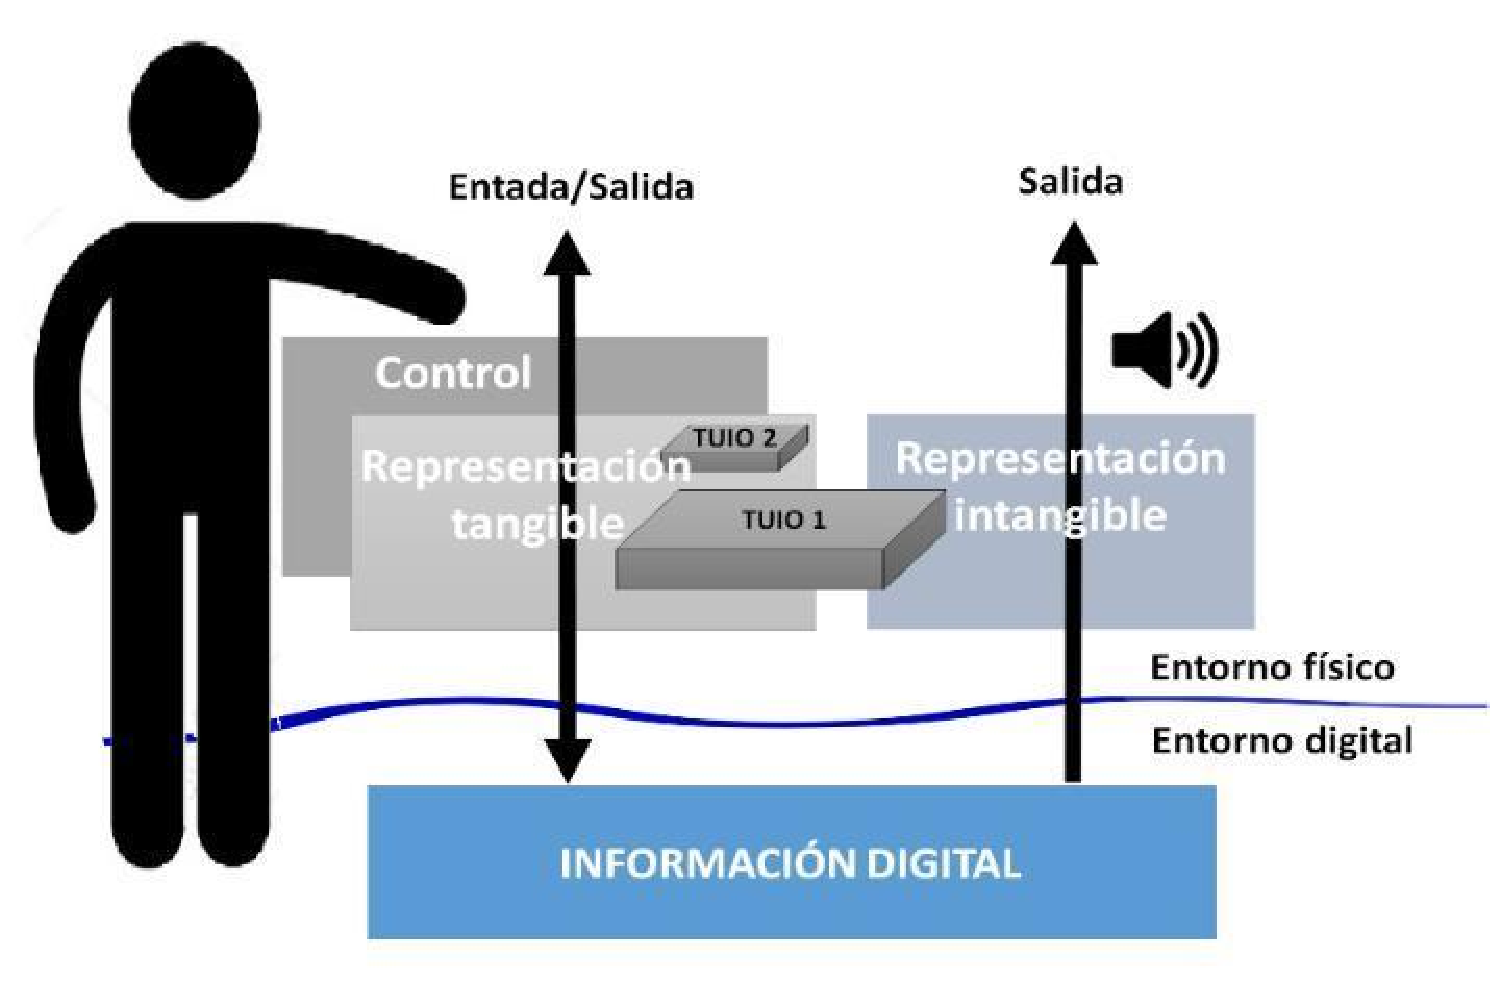
\includegraphics[width=0.5\textwidth]{SIS.pdf}
\caption{Modelo de interacción de interfaz TUI para este proyecto}
\label{fig:SIS}
\end{center}
\end{figure}

El sistema de juego propuesto abarca desde el desarrollo de una secuencia, a partir de los criterios de creación del niño, hasta la resolución de pequeños problemas de lógica. El elemento \emph{TUIO1} consta de una pantalla táctil, encargada de la representación gráfica tangible e intangible del juego. Si bien los elementos tangibles juegan el papel central en la representación y control en un \emph{TUI}, la representación intangible es también importante, añadiendo gráficos y audio, siendo esta información dinámica proporcionada, una gran ayuda a la hora de realizar la interacción. 

La existencia en tiempo real de una realimentación de la representación intangible, cuando se ha manipulado la representación tangible, es fundamental para asegurar un correcto acoplamiento perceptivo. Las representaciones intangibles que incorpora el diseño son tanto auditivas, producidas en determinados puntos del desarrollo del juego, como gráficas, mostrando en determinadas zonas de la pantalla táctil, información no modificable por el usuario.
Los componentes, y los eventos que se producen en la interacción, junto con las comunicaciones con \emph{TUIO2}, están controladas mediante un microprocesador.

El segundo elemento tangible \emph{TUIO2}, actúa como elemento de programación tangible, agrupando funciones,
características y elementos que pueden ser aplicados al juego, y que facilitan las interacciones o modificaciones a efectuar sobre el juego. Uno de los factores principales de las interfaces tangibles, es el acoplamiento de las representaciones tangibles a información digital y modelos computacionales. 

Uno de los retos en el diseño de \emph{TUI}, es como \emph{mapear} los objetos físicos y como realizar una manipulación a la computación digital y la retroalimentación de una manera significativa y completa.
Para solucionar el problema de disponer de distintos elementos tangibles para el desarrollo del juego, el dispositivo \emph{TUIO2} hace de puente entre la interfaz física y la digital, agrupando todos los elementos de interacción en un solo dispositivo. 

Al disponer de una pantalla táctil se hace más intuitivo y sencillo el uso de este elemento tangible. Además de una pantalla táctil dispone de sensores de posicionamiento y orientación. Estos componentes y los eventos producidos son tratados en un microcontrolador, el cual también es el encargado de las comunicaciones con el dispositivo \emph{TUIO1}.


\section{Estructura del documento}

A continuación, se describe la estructura de contenidos que se ha seguido en el presente documento y que consta de ocho capítulos:
\textbf{Capítulo 2: Objetivos}\\
Este capítulo se detalla los principales objetivos del TFG, indicando cuales son los requisitos mínimos que debe cumplir el software de la aplicación. 

\textbf{Capítulo 3: Antecedentes}\\
En este capítulo se muestran los resultados sobre los principales estudios experimentales aplicados a la interacción tangible, y como motiva a niños de tempranas edades en sus habilidades computacionales, además de las ventajas en el aprendizaje mientras manipulan objetos en el escenario educativo.
Se muestran algunos de los dispositivos más importantes y los diferentes enfoques que aportan en la interacción tangible aplicados al aprendizaje computacional, así como sus características y tecnología utilizada.
También son mencionados los dispositivos con aplicaciones multipantalla, ya que algunas de sus características son aplicadas en el presente TFG.

\textbf{Capítulo 4: Interacción Persona-Ordenador e Interfaces}\\
La finalidad del capítulo es introducir una visión más amplia de la interacción Persona-Ordenador, describiendo sus principales características, y como las interfaces han ido evolucionando. Se analizan las ventajas y restricciones de cada una de ellas a la hora de adaptarse a distintos entornos y situaciones. Las interfaces tratadas en este capítulo son:
\begin{itemize}
\item Interfaz Gráfica de Usuario (GUI).
\item Interfaz de Usuario Tangible (TUI), y su uso en la educación.
\item Interfaz Sistema Multipantalla.
\item Pantallas capacitivas. Funcionamiento \emph{Widgets Capacitivos}.
\end{itemize}

\textbf{Capítulo 5: Tecnologías para el desarrollo. Hardware y Software.}\\
Este capítulo explica las funciones y características, de cada uno de los elementos hardware utilizados para realizar la plataforma de juego, así como el conjunto de herramientas software aplicadas para desarrollar los programas que manejan la plataforma.

\textbf{Capítulo 6: Método de trabajo}\\
Exposición y planteamiento del método de trabajo seguido para desarrollar la aplicación. Se ha aplicado la metodología de desarrollo \textbf{SCRUM}. En este capitulo son explicados cada uno de los pasos que han sido necesarios para realizar la plataforma de juego.


\textbf{Capítulo 7: Resultados}\\
En este capítulo se presentan los resultados obtenidos en el desarrollo de la aplicación, explicando la evolución por aspectos, comunicaciones, software de la interfaz gráfica, etc..

\textbf{Capítulo 8: Conclusiones}\\




% Local Variables:
%  coding: utf-8
%  mode: latex
%  mode: flyspell
%  ispell-local-dictionary: "castellano8"
% End:

